% Options for packages loaded elsewhere
\PassOptionsToPackage{unicode}{hyperref}
\PassOptionsToPackage{hyphens}{url}
%
\documentclass[
]{article}
\usepackage{amsmath,amssymb}
\usepackage{iftex}
\ifPDFTeX
  \usepackage[T1]{fontenc}
  \usepackage[utf8]{inputenc}
  \usepackage{textcomp} % provide euro and other symbols
\else % if luatex or xetex
  \usepackage{unicode-math} % this also loads fontspec
  \defaultfontfeatures{Scale=MatchLowercase}
  \defaultfontfeatures[\rmfamily]{Ligatures=TeX,Scale=1}
\fi
\usepackage{lmodern}
\ifPDFTeX\else
  % xetex/luatex font selection
\fi
% Use upquote if available, for straight quotes in verbatim environments
\IfFileExists{upquote.sty}{\usepackage{upquote}}{}
\IfFileExists{microtype.sty}{% use microtype if available
  \usepackage[]{microtype}
  \UseMicrotypeSet[protrusion]{basicmath} % disable protrusion for tt fonts
}{}
\makeatletter
\@ifundefined{KOMAClassName}{% if non-KOMA class
  \IfFileExists{parskip.sty}{%
    \usepackage{parskip}
  }{% else
    \setlength{\parindent}{0pt}
    \setlength{\parskip}{6pt plus 2pt minus 1pt}}
}{% if KOMA class
  \KOMAoptions{parskip=half}}
\makeatother
\usepackage{xcolor}
\usepackage[margin=1in]{geometry}
\usepackage{color}
\usepackage{fancyvrb}
\newcommand{\VerbBar}{|}
\newcommand{\VERB}{\Verb[commandchars=\\\{\}]}
\DefineVerbatimEnvironment{Highlighting}{Verbatim}{commandchars=\\\{\}}
% Add ',fontsize=\small' for more characters per line
\usepackage{framed}
\definecolor{shadecolor}{RGB}{248,248,248}
\newenvironment{Shaded}{\begin{snugshade}}{\end{snugshade}}
\newcommand{\AlertTok}[1]{\textcolor[rgb]{0.94,0.16,0.16}{#1}}
\newcommand{\AnnotationTok}[1]{\textcolor[rgb]{0.56,0.35,0.01}{\textbf{\textit{#1}}}}
\newcommand{\AttributeTok}[1]{\textcolor[rgb]{0.13,0.29,0.53}{#1}}
\newcommand{\BaseNTok}[1]{\textcolor[rgb]{0.00,0.00,0.81}{#1}}
\newcommand{\BuiltInTok}[1]{#1}
\newcommand{\CharTok}[1]{\textcolor[rgb]{0.31,0.60,0.02}{#1}}
\newcommand{\CommentTok}[1]{\textcolor[rgb]{0.56,0.35,0.01}{\textit{#1}}}
\newcommand{\CommentVarTok}[1]{\textcolor[rgb]{0.56,0.35,0.01}{\textbf{\textit{#1}}}}
\newcommand{\ConstantTok}[1]{\textcolor[rgb]{0.56,0.35,0.01}{#1}}
\newcommand{\ControlFlowTok}[1]{\textcolor[rgb]{0.13,0.29,0.53}{\textbf{#1}}}
\newcommand{\DataTypeTok}[1]{\textcolor[rgb]{0.13,0.29,0.53}{#1}}
\newcommand{\DecValTok}[1]{\textcolor[rgb]{0.00,0.00,0.81}{#1}}
\newcommand{\DocumentationTok}[1]{\textcolor[rgb]{0.56,0.35,0.01}{\textbf{\textit{#1}}}}
\newcommand{\ErrorTok}[1]{\textcolor[rgb]{0.64,0.00,0.00}{\textbf{#1}}}
\newcommand{\ExtensionTok}[1]{#1}
\newcommand{\FloatTok}[1]{\textcolor[rgb]{0.00,0.00,0.81}{#1}}
\newcommand{\FunctionTok}[1]{\textcolor[rgb]{0.13,0.29,0.53}{\textbf{#1}}}
\newcommand{\ImportTok}[1]{#1}
\newcommand{\InformationTok}[1]{\textcolor[rgb]{0.56,0.35,0.01}{\textbf{\textit{#1}}}}
\newcommand{\KeywordTok}[1]{\textcolor[rgb]{0.13,0.29,0.53}{\textbf{#1}}}
\newcommand{\NormalTok}[1]{#1}
\newcommand{\OperatorTok}[1]{\textcolor[rgb]{0.81,0.36,0.00}{\textbf{#1}}}
\newcommand{\OtherTok}[1]{\textcolor[rgb]{0.56,0.35,0.01}{#1}}
\newcommand{\PreprocessorTok}[1]{\textcolor[rgb]{0.56,0.35,0.01}{\textit{#1}}}
\newcommand{\RegionMarkerTok}[1]{#1}
\newcommand{\SpecialCharTok}[1]{\textcolor[rgb]{0.81,0.36,0.00}{\textbf{#1}}}
\newcommand{\SpecialStringTok}[1]{\textcolor[rgb]{0.31,0.60,0.02}{#1}}
\newcommand{\StringTok}[1]{\textcolor[rgb]{0.31,0.60,0.02}{#1}}
\newcommand{\VariableTok}[1]{\textcolor[rgb]{0.00,0.00,0.00}{#1}}
\newcommand{\VerbatimStringTok}[1]{\textcolor[rgb]{0.31,0.60,0.02}{#1}}
\newcommand{\WarningTok}[1]{\textcolor[rgb]{0.56,0.35,0.01}{\textbf{\textit{#1}}}}
\usepackage{graphicx}
\makeatletter
\def\maxwidth{\ifdim\Gin@nat@width>\linewidth\linewidth\else\Gin@nat@width\fi}
\def\maxheight{\ifdim\Gin@nat@height>\textheight\textheight\else\Gin@nat@height\fi}
\makeatother
% Scale images if necessary, so that they will not overflow the page
% margins by default, and it is still possible to overwrite the defaults
% using explicit options in \includegraphics[width, height, ...]{}
\setkeys{Gin}{width=\maxwidth,height=\maxheight,keepaspectratio}
% Set default figure placement to htbp
\makeatletter
\def\fps@figure{htbp}
\makeatother
\setlength{\emergencystretch}{3em} % prevent overfull lines
\providecommand{\tightlist}{%
  \setlength{\itemsep}{0pt}\setlength{\parskip}{0pt}}
\setcounter{secnumdepth}{-\maxdimen} % remove section numbering
\ifLuaTeX
  \usepackage{selnolig}  % disable illegal ligatures
\fi
\usepackage{bookmark}
\IfFileExists{xurl.sty}{\usepackage{xurl}}{} % add URL line breaks if available
\urlstyle{same}
\hypersetup{
  pdftitle={LAB\_03},
  pdfauthor={Ryan Waterman},
  hidelinks,
  pdfcreator={LaTeX via pandoc}}

\title{LAB\_03}
\author{Ryan Waterman}
\date{2025-01-20}

\begin{document}
\maketitle

\section{LAB 3}\label{lab-3}

Imports:

\begin{Shaded}
\begin{Highlighting}[]
\FunctionTok{library}\NormalTok{(tidyverse)}
\end{Highlighting}
\end{Shaded}

\begin{verbatim}
## -- Attaching core tidyverse packages ------------------------ tidyverse 2.0.0 --
## v dplyr     1.1.4     v readr     2.1.5
## v forcats   1.0.0     v stringr   1.5.1
## v ggplot2   3.5.1     v tibble    3.2.1
## v lubridate 1.9.4     v tidyr     1.3.1
## v purrr     1.0.2     
## -- Conflicts ------------------------------------------ tidyverse_conflicts() --
## x dplyr::filter() masks stats::filter()
## x dplyr::lag()    masks stats::lag()
## i Use the conflicted package (<http://conflicted.r-lib.org/>) to force all conflicts to become errors
\end{verbatim}

\begin{Shaded}
\begin{Highlighting}[]
\FunctionTok{library}\NormalTok{(ggplot2)}
\FunctionTok{library}\NormalTok{(dplyr)}
\end{Highlighting}
\end{Shaded}

\subsection{1.4 Buteyko method, study
components}\label{buteyko-method-study-components}

\begin{quote}
The Buteyko method is a shallow breathing technique developed by
Konstantin Buteyko, a Russian doctor, in 1952. Anecdotal evidence
suggests that the Buteyko method can reduce asthma symptoms and improve
quality of life. In a scientific study to determine the effectiveness of
this method, researchers recruited 600 asthma patients aged 18-69 who
relied on medication for asthma treatment. These patients were randomly
split into two research groups: one practiced the Buteyko method and the
other did not. Patients were scored on quality of life, activity, asthma
symptoms, and medication reduction on a scale from 0 to 10. On average,
the participants in the Buteyko group experienced a significant
reduction in asthma symptoms and an improvement in quality of life.
\end{quote}

\subsubsection{(a) Identify the main research question of the
study.}\label{a-identify-the-main-research-question-of-the-study.}

\emph{The main research question is whether the Buteyko method is an
effective way to reduce asthma symptoms.}

\subsubsection{(b) Who are the subjects in this study, and how many are
included?}\label{b-who-are-the-subjects-in-this-study-and-how-many-are-included}

\subsubsection{(c) What are the variables in the study? Identify each
variable as numerical or categorical. If numerical, state whether the
variable is discrete or continuous. If categorical, state whether the
variable is
ordinal.}\label{c-what-are-the-variables-in-the-study-identify-each-variable-as-numerical-or-categorical.-if-numerical-state-whether-the-variable-is-discrete-or-continuous.-if-categorical-state-whether-the-variable-is-ordinal.}

\subsection{1.6 Stealers, study
components}\label{stealers-study-components}

\begin{quote}
In a study of the relationship between socio-economic class and
unethical behavior, 129 University of California undergraduates at
Berkeley were asked to identify themselves as having low or high
social-class by comparing themselves to others with the most (least)
money, most (least) education, and most (least) respected jobs. They
were also presented with a jar of individually wrapped candies and
informed that the candies were for children in a nearby laboratory, but
that they could take some if they wanted. After completing some
unrelated tasks, participants reported the number of candies they had
taken.
\end{quote}

\subsubsection{(a) Identify the main research question of the
study.}\label{a-identify-the-main-research-question-of-the-study.-1}

\subsubsection{(b) Who are the subjects in this study, and how many are
included?}\label{b-who-are-the-subjects-in-this-study-and-how-many-are-included-1}

\subsubsection{(c) The study found that students who were identified as
upper-class took more candy than others. How many variables were
recorded for each subject in the study in order to conclude these
findings? State the variables and their
types.}\label{c-the-study-found-that-students-who-were-identified-as-upper-class-took-more-candy-than-others.-how-many-variables-were-recorded-for-each-subject-in-the-study-in-order-to-conclude-these-findings-state-the-variables-and-their-types.}

\subsection{1.12 UN Votes}\label{un-votes}

\begin{quote}
The visualization below shows voting patterns in the United States,
Canada, and Mexico in the United Nations General Assembly on a variety
of issues. Specifically, for a given year between 1946 and 2015, it
displays the percentage of roll calls in which the country voted yes for
each issue. This visualization was constructed based on a dataset where
each observation is a country/year pair.
\end{quote}

\begin{figure}
\centering
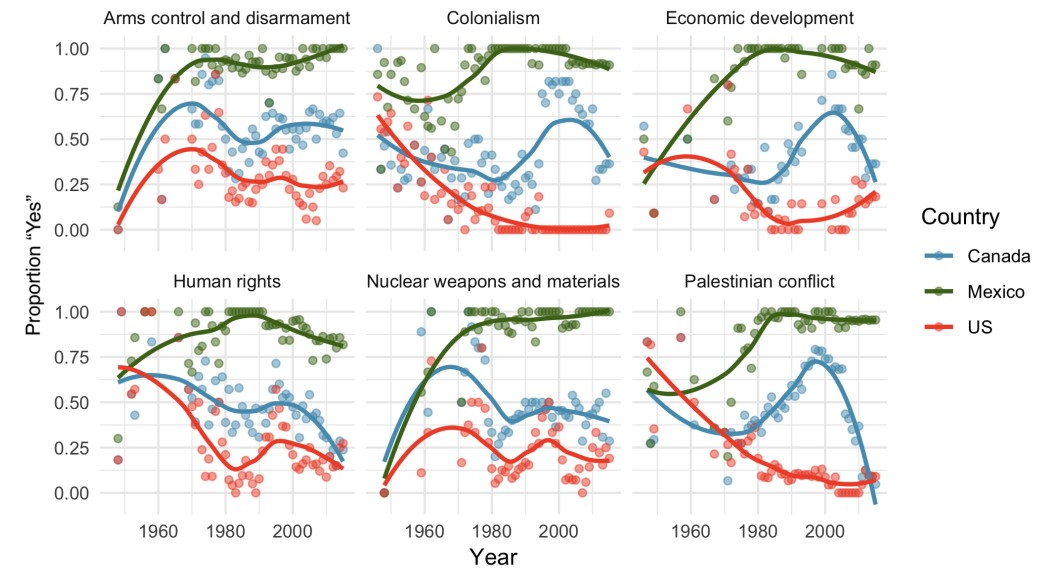
\includegraphics{./assets/1-12.jpg}
\caption{Figure 1-12}
\end{figure}

\subsubsection{(a) List the variables used in creating this
visualization.}\label{a-list-the-variables-used-in-creating-this-visualization.}

\subsubsection{(b) Indicate whether each variable in the study is
numerical or categorical. If numerical, identify as continuous or
discrete. If categorical, indicate if the variable is
ordinal.}\label{b-indicate-whether-each-variable-in-the-study-is-numerical-or-categorical.-if-numerical-identify-as-continuous-or-discrete.-if-categorical-indicate-if-the-variable-is-ordinal.}

\subsection{1.18 Cats on YouTube}\label{cats-on-youtube}

\begin{quote}
Suppose you want to estimate the percentage of videos on YouTube that
are cat videos. It is impossible for you to watch all videos on YouTube
so you use a random video picker to select 1000 videos for you. You find
that 2\% of these videos are cat videos. Determine which of the
following is an observation, a variable, a sample statistic (value
calculated based on the observed sample), or a population parameter.
\end{quote}

\subsubsection{(a) Percentage of all videos on YouTube that are cat
videos.}\label{a-percentage-of-all-videos-on-youtube-that-are-cat-videos.}

\subsubsection{(b) 2\%.}\label{b-2.}

\subsubsection{(c) A video in your
sample.}\label{c-a-video-in-your-sample.}

\subsubsection{(d) Whether or not a video is a cat
video.}\label{d-whether-or-not-a-video-is-a-cat-video.}

\subsection{1.20 Housing proposal across
dorms}\label{housing-proposal-across-dorms}

\begin{quote}
On a large college campus first-year students and sophomores live in
dorms located on the eastern part of the campus and juniors and seniors
live in dorms located on the western part of the campus. Suppose you
want to collect student opinions on a new housing structure the college
administration is proposing and you want to make sure your survey
equally represents opinions from students from all years.
\end{quote}

\subsubsection{(a) What type of study is
this?}\label{a-what-type-of-study-is-this}

\subsubsection{(b) Suggest a sampling strategy for carrying out this
study}\label{b-suggest-a-sampling-strategy-for-carrying-out-this-study}

\subsection{1.34 Exercise and mental
health}\label{exercise-and-mental-health}

\begin{quote}
A researcher is interested in the effects of exercise on mental health
and he proposes the following study: Use stratified random sampling to
ensure representative proportions of 18-30, 31-40 and 41- 55 year olds
from the population. Next, randomly assign half the subjects from each
age group to exercise twice a week, and instruct the rest not to
exercise. Conduct a mental health exam at the beginning and at the end
of the study, and compare the results.
\end{quote}

\subsubsection{(a) What type of study is
this?}\label{a-what-type-of-study-is-this-1}

\subsubsection{(b) What are the treatment and control groups in this
study?}\label{b-what-are-the-treatment-and-control-groups-in-this-study}

\subsubsection{(c) Does this study make use of blocking? If so, what is
the blocking
variable?}\label{c-does-this-study-make-use-of-blocking-if-so-what-is-the-blocking-variable}

\subsubsection{(d) Does this study make use of
blinding?}\label{d-does-this-study-make-use-of-blinding}

\subsubsection{(e) Comment on whether or not the results of the study
can be used to establish a causal relationship between exercise and
mental health, and indicate whether or not the conclusions can be
generalized to the population at
large.}\label{e-comment-on-whether-or-not-the-results-of-the-study-can-be-used-to-establish-a-causal-relationship-between-exercise-and-mental-health-and-indicate-whether-or-not-the-conclusions-can-be-generalized-to-the-population-at-large.}

\subsubsection{(f) Suppose you are given the task of determining if this
proposed study should get funding. Would you have any reservations about
the study
proposal?}\label{f-suppose-you-are-given-the-task-of-determining-if-this-proposed-study-should-get-funding.-would-you-have-any-reservations-about-the-study-proposal}

\subsection{2.2 Associations.}\label{associations.}

\begin{quote}
Indicate which of the plots show:
\end{quote}

\subsubsection{(a) a positive
association}\label{a-a-positive-association}

\subsubsection{(b) a negative
association}\label{b-a-negative-association}

\subsubsection{(c) no association.}\label{c-no-association.}

\subsubsection{(d) Also determine if the positive and negative
associations are linear or nonlinear. Each part may refer to more than
one
plot.}\label{d-also-determine-if-the-positive-and-negative-associations-are-linear-or-nonlinear.-each-part-may-refer-to-more-than-one-plot.}

\begin{figure}
\centering
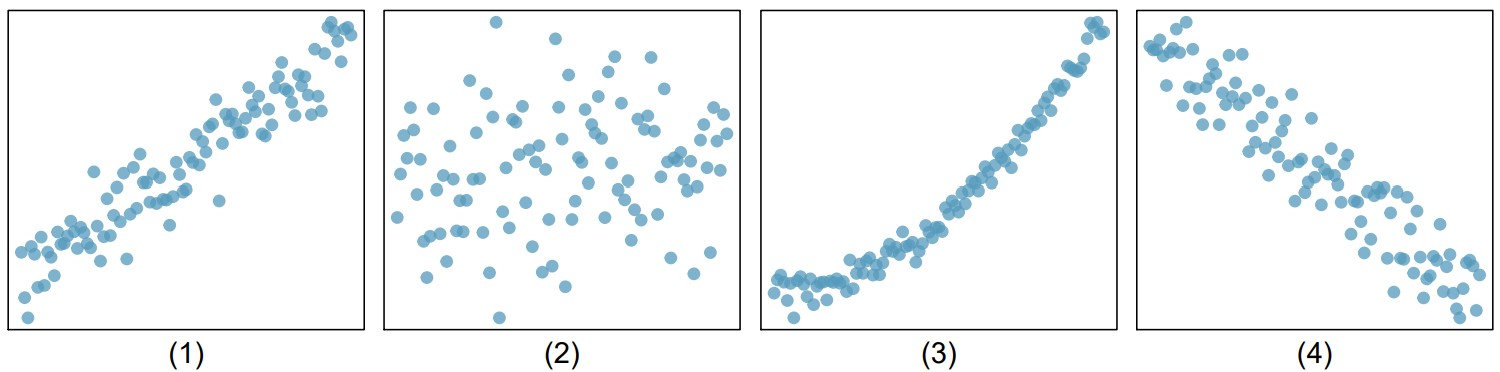
\includegraphics{./assets/2-2.jpg}
\caption{Figure 2-2}
\end{figure}

\subsection{2.6 Sleeping in college}\label{sleeping-in-college}

\begin{quote}
A recent article in a college newspaper stated that college students get
an average of 5.5 hrs of sleep each night. A student who was skeptical
about this value decided to conduct a survey by randomly sampling 25
students. On average, the sampled students slept 6.25 hours per night.
Identify which value represents the sample mean and which value
represents the claimed population mean.
\end{quote}

\subsection{2.10 Mix-and-match}\label{mix-and-match}

\begin{quote}
Describe the distribution in the histograms below and match them to the
box plots.
\end{quote}

\begin{figure}
\centering
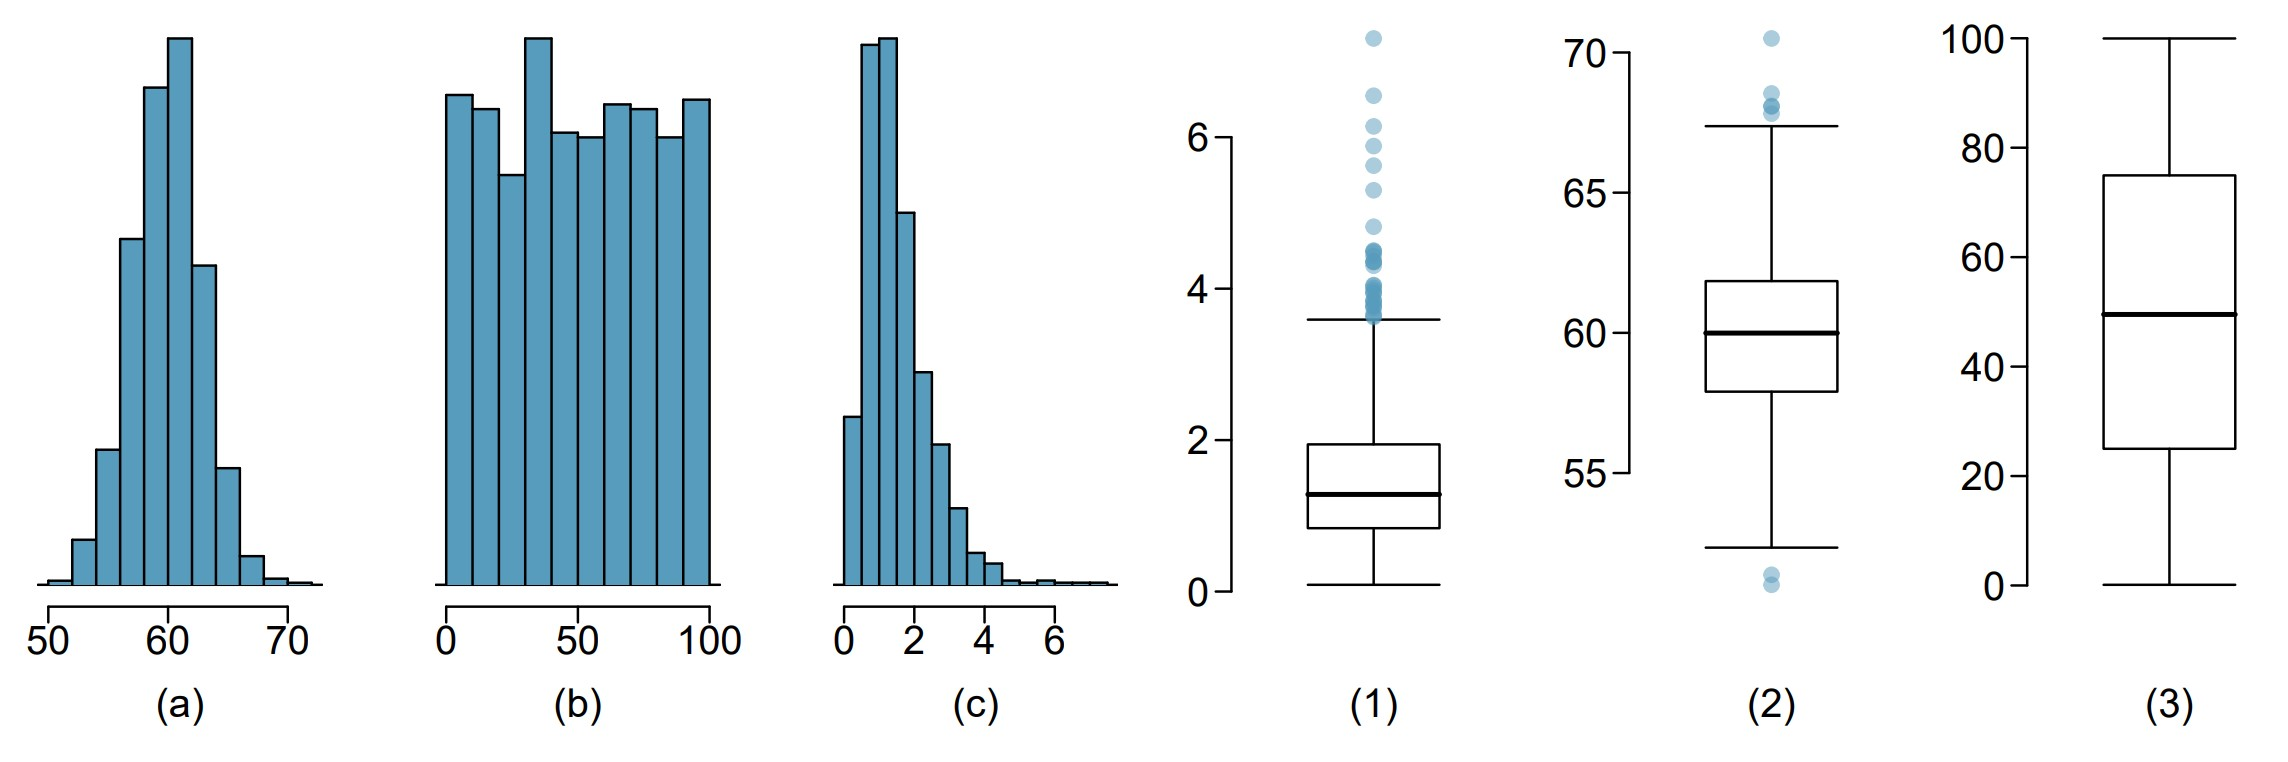
\includegraphics{./assets/2-10.jpg}
\caption{Figure 2-10}
\end{figure}

\subsection{2.12 Median vs.~mean}\label{median-vs.-mean}

\begin{quote}
Estimate the median for the 400 observations shown in the histogram, and
note whether you expect the mean to be higher or lower than the median.
\end{quote}

\begin{figure}
\centering
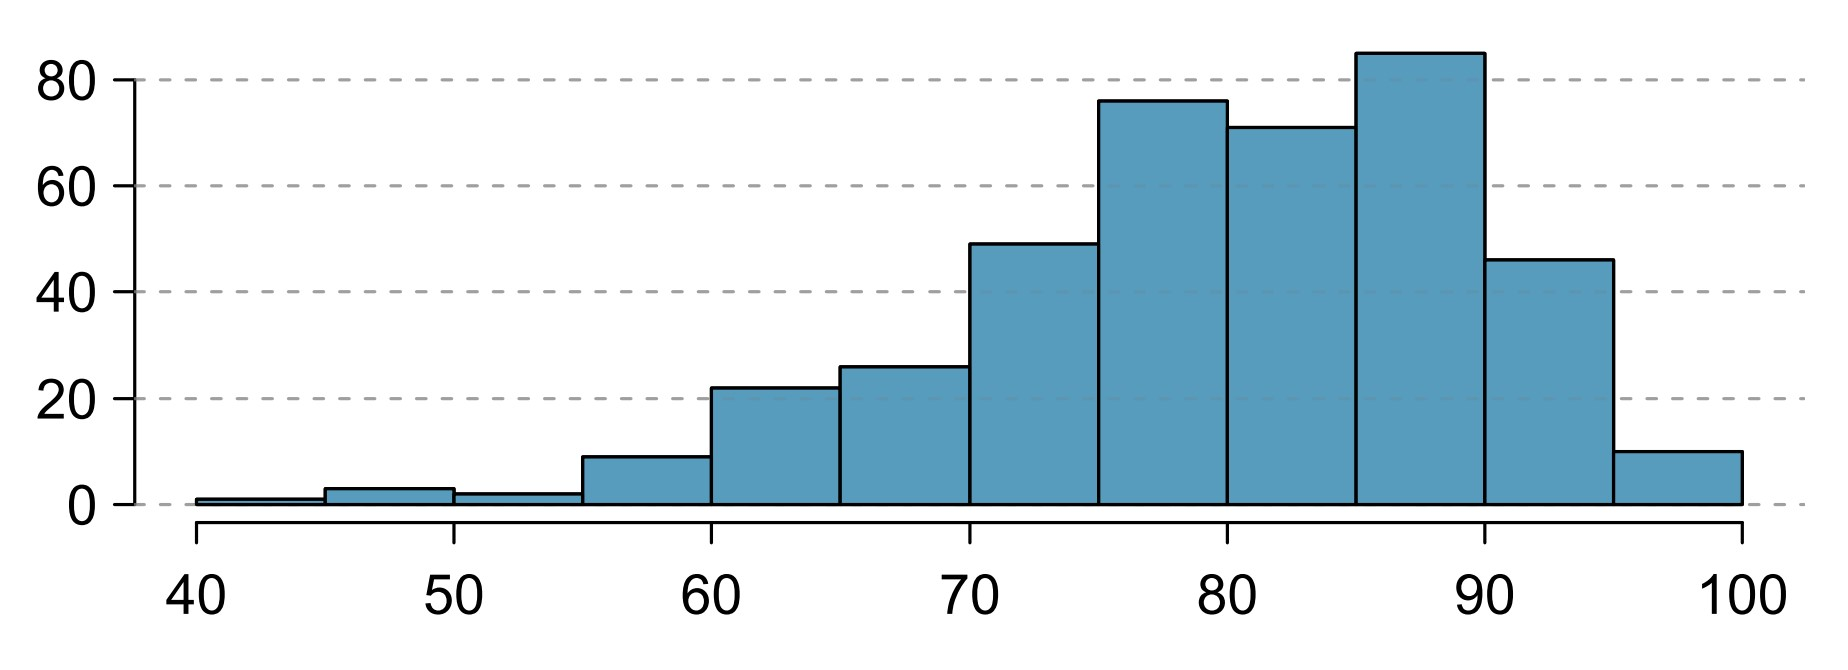
\includegraphics{./assets/2-12.jpg}
\caption{Figure 2-12}
\end{figure}

\subsection{2.16 Distributions and appropriate statistics, Part
II}\label{distributions-and-appropriate-statistics-part-ii}

\begin{quote}
For each of the following, state whether you expect the distribution to
be symmetric, right skewed, or left skewed. Also specify whether the
mean or median would best represent a typical observation in the data,
and whether the variability of observations would be best represented
using the standard deviation or IQR. Explain your reasoning.
\end{quote}

\subsubsection{(a) Housing prices in a country where 25\% of the houses
cost below \$350,000, 50\% of the houses cost below \$450,000, 75\% of
the houses cost below \$1,000,000 and there are a meaningful number of
houses that cost more than
\$6,000,000.}\label{a-housing-prices-in-a-country-where-25-of-the-houses-cost-below-350000-50-of-the-houses-cost-below-450000-75-of-the-houses-cost-below-1000000-and-there-are-a-meaningful-number-of-houses-that-cost-more-than-6000000.}

\subsubsection{(b) Housing prices in a country where 25\% of the houses
cost below \$300,000, 50\% of the houses cost below \$600,000, 75\% of
the houses cost below \$900,000 and very few houses that cost more than
\$1,200,000.}\label{b-housing-prices-in-a-country-where-25-of-the-houses-cost-below-300000-50-of-the-houses-cost-below-600000-75-of-the-houses-cost-below-900000-and-very-few-houses-that-cost-more-than-1200000.}

\subsubsection{(c) Number of alcoholic drinks consumed by college
students in a given week. Assume that most of these students don't drink
since they are under 21 years old, and only a few drink
excessively.}\label{c-number-of-alcoholic-drinks-consumed-by-college-students-in-a-given-week.-assume-that-most-of-these-students-dont-drink-since-they-are-under-21-years-old-and-only-a-few-drink-excessively.}

\subsubsection{(d) Annual salaries of the employees at a Fortune 500
company where only a few high level executives earn much higher salaries
than all the other
employees.}\label{d-annual-salaries-of-the-employees-at-a-fortune-500-company-where-only-a-few-high-level-executives-earn-much-higher-salaries-than-all-the-other-employees.}

\subsection{2.20 Hispanic population}\label{hispanic-population}

\begin{quote}
The US census collects data on race and ethnicity of Americans, among
many other variables. The histogram below shows the distribution of the
percentage of the population that is Hispanic in 3,142 counties in the
US in 2010. Also shown is a histogram of logs of these values.
\end{quote}

\begin{figure}
\centering
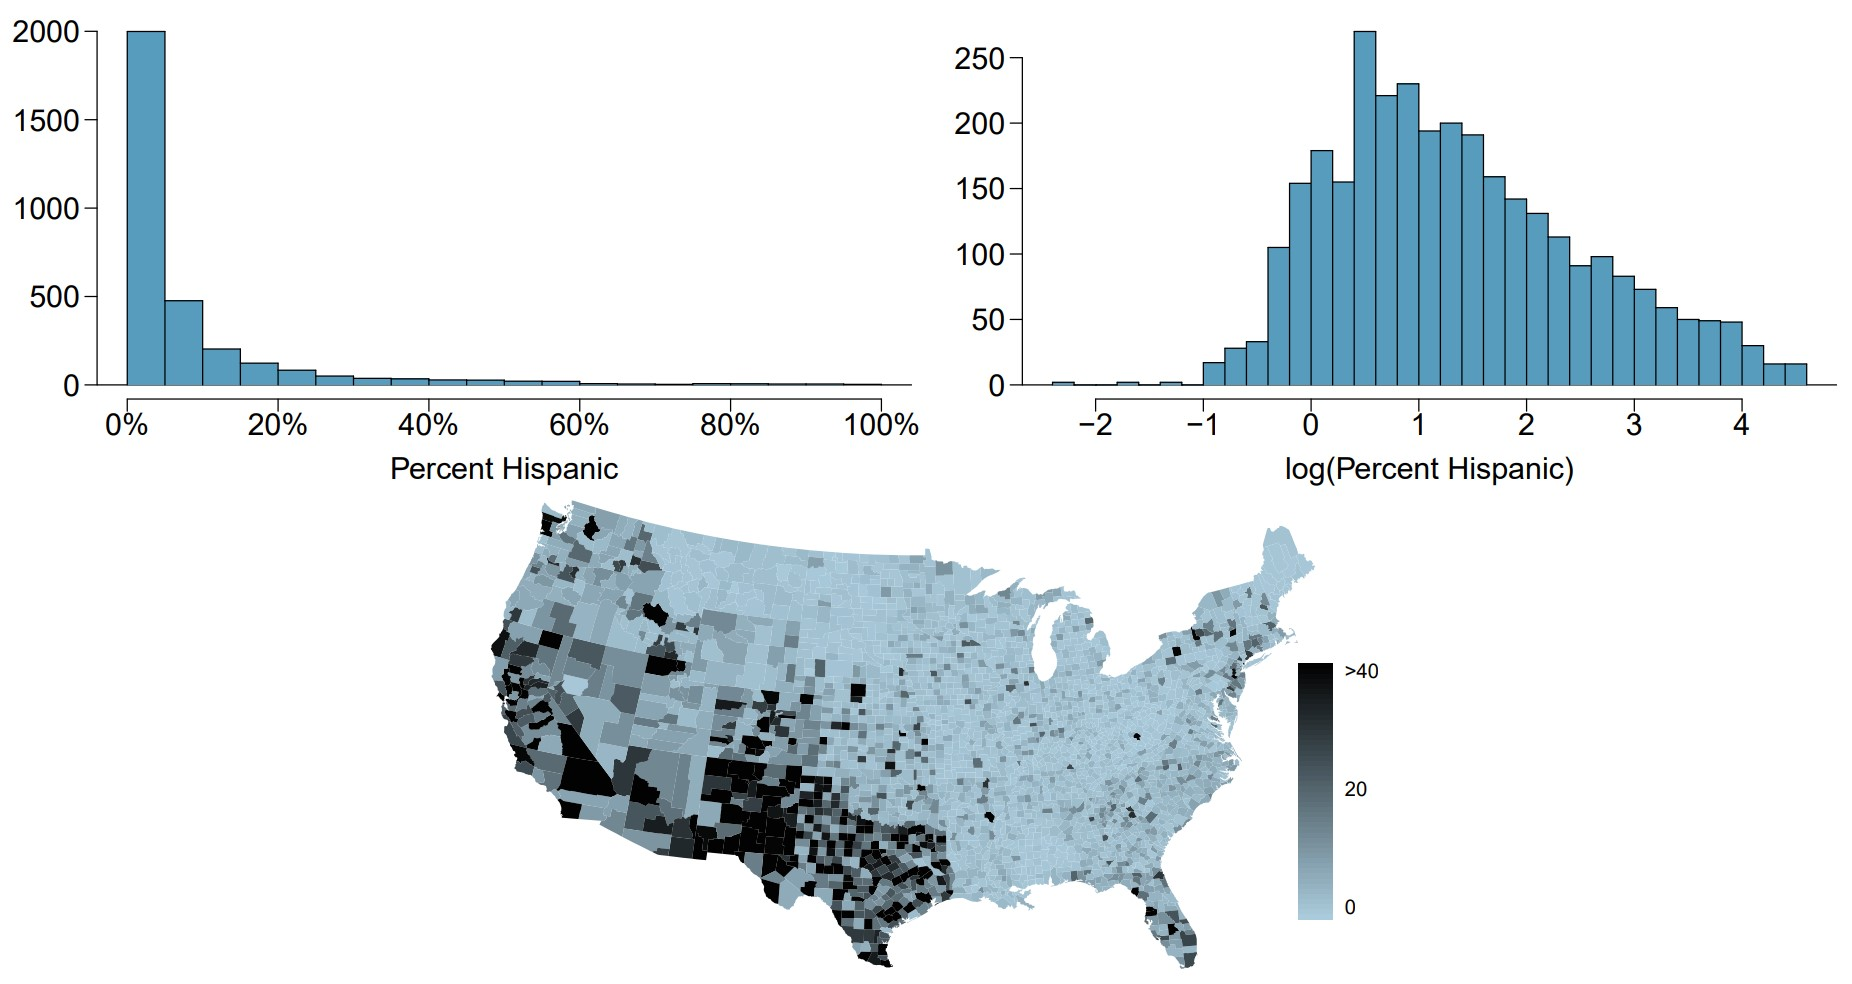
\includegraphics{./assets/2-20.jpg}
\caption{Figure 2-20}
\end{figure}

\subsubsection{(a) Describe the numerical distribution and comment on
why we might want to use log-transformed values in analyzing or modeling
these
data.}\label{a-describe-the-numerical-distribution-and-comment-on-why-we-might-want-to-use-log-transformed-values-in-analyzing-or-modeling-these-data.}

\subsubsection{(b) What features of the distribution of the Hispanic
population in US counties are apparent in the map but not in the
histogram? What features are apparent in the histogram but not the
map?}\label{b-what-features-of-the-distribution-of-the-hispanic-population-in-us-counties-are-apparent-in-the-map-but-not-in-the-histogram-what-features-are-apparent-in-the-histogram-but-not-the-map}

\subsubsection{(c) Is one visualization more appropriate or helpful than
the other? Explain your
reasoning.}\label{c-is-one-visualization-more-appropriate-or-helpful-than-the-other-explain-your-reasoning.}

\subsection{2.22 Views on immigration}\label{views-on-immigration}

\begin{quote}
910 randomly sampled registered voters from Tampa, FL were asked if they
thought workers who have illegally entered the US should be (i) allowed
to keep their jobs and apply for US citizenship, (ii) allowed to keep
their jobs as temporary guest workers but not allowed to apply for US
citizenship, or (iii) lose their jobs and have to leave the country. The
results of the survey by political ideology are shown below.
\end{quote}

\begin{figure}
\centering
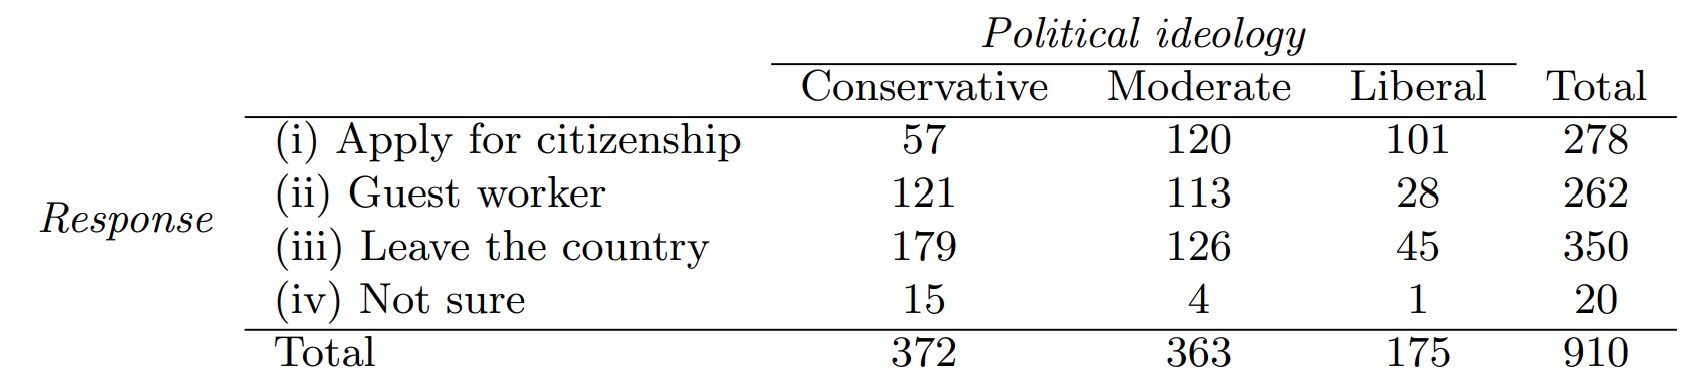
\includegraphics{./assets/2-22.jpg}
\caption{Figure 2-22}
\end{figure}

\subsubsection{(a) What percent of these Tampa, FL voters identify
themselves as
conservatives?}\label{a-what-percent-of-these-tampa-fl-voters-identify-themselves-as-conservatives}

\subsubsection{(b) What percent of these Tampa, FL voters are in favor
of the citizenship
option?}\label{b-what-percent-of-these-tampa-fl-voters-are-in-favor-of-the-citizenship-option}

\subsubsection{(c) What percent of these Tampa, FL voters identify
themselves as conservatives and are in favor of the citizenship
option?}\label{c-what-percent-of-these-tampa-fl-voters-identify-themselves-as-conservatives-and-are-in-favor-of-the-citizenship-option}

\subsubsection{(d) What percent of these Tampa, FL voters who identify
themselves as conservatives are also in favor of the citizenship option?
What percent of moderates share this view? What percent of liberals
share this
view?}\label{d-what-percent-of-these-tampa-fl-voters-who-identify-themselves-as-conservatives-are-also-in-favor-of-the-citizenship-option-what-percent-of-moderates-share-this-view-what-percent-of-liberals-share-this-view}

\subsubsection{(e) Do political ideology and views on immigration appear
to be independent? Explain your
reasoning.}\label{e-do-political-ideology-and-views-on-immigration-appear-to-be-independent-explain-your-reasoning.}

\subsection{2.24 Raise taxes}\label{raise-taxes}

\begin{quote}
A random sample of registered voters nationally were asked whether they
think it's better to raise taxes on the rich or raise taxes on the poor.
The survey also collected information on the political party affiliation
of the respondents. Based on the mosaic plot shown below, do views on
raising taxes and political affiliation appear to be independent?
Explain your reasoning.
\end{quote}

\begin{figure}
\centering
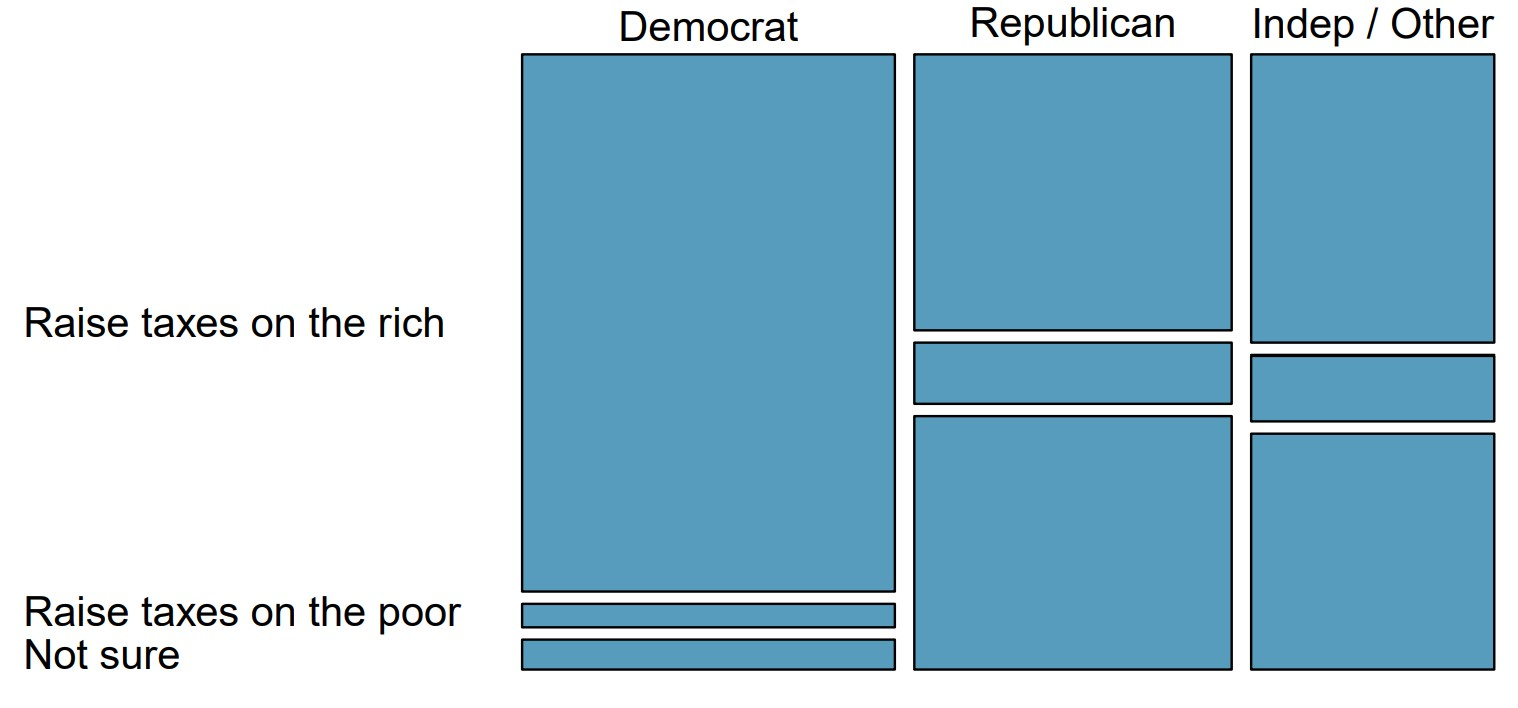
\includegraphics{./assets/2-24.jpg}
\caption{Figure 2-24}
\end{figure}

\subsection{Question 2A - Correlation}\label{question-2a---correlation}

\begin{Shaded}
\begin{Highlighting}[]
\FunctionTok{require}\NormalTok{(maps)}
\end{Highlighting}
\end{Shaded}

\begin{verbatim}
## Loading required package: maps
\end{verbatim}

\begin{verbatim}
## 
## Attaching package: 'maps'
\end{verbatim}

\begin{verbatim}
## The following object is masked from 'package:purrr':
## 
##     map
\end{verbatim}

\begin{Shaded}
\begin{Highlighting}[]
\FunctionTok{head}\NormalTok{(state.x77)}
\end{Highlighting}
\end{Shaded}

\begin{verbatim}
##            Population Income Illiteracy Life Exp Murder HS Grad Frost   Area
## Alabama          3615   3624        2.1    69.05   15.1    41.3    20  50708
## Alaska            365   6315        1.5    69.31   11.3    66.7   152 566432
## Arizona          2212   4530        1.8    70.55    7.8    58.1    15 113417
## Arkansas         2110   3378        1.9    70.66   10.1    39.9    65  51945
## California      21198   5114        1.1    71.71   10.3    62.6    20 156361
## Colorado         2541   4884        0.7    72.06    6.8    63.9   166 103766
\end{verbatim}

\begin{Shaded}
\begin{Highlighting}[]
\NormalTok{state\_df}\OtherTok{=}\FunctionTok{data.frame}\NormalTok{(state.x77)}
\end{Highlighting}
\end{Shaded}

\begin{quote}
In this data set, we have data about US states in 1975, so this is old
data. We have variables that relate to life experiences: Income,
illiteracy, life expectancy, HS Graduation rate. These are rates over
the population of a state. State your answers, then compute the
correlation and explain what the answer means.
\end{quote}

\subsubsection{(a) Which of these would you expect to have high positive
correlation?}\label{a-which-of-these-would-you-expect-to-have-high-positive-correlation}

\subsubsection{(b) Which pair would you expect to be most highly
correlated?}\label{b-which-pair-would-you-expect-to-be-most-highly-correlated}

\subsubsection{(c) Which pair would have the most negative
correlation?}\label{c-which-pair-would-have-the-most-negative-correlation}

\begin{Shaded}
\begin{Highlighting}[]
\CommentTok{\#your code here}
\end{Highlighting}
\end{Shaded}

\subsubsection{(d) Create a correlation matrix of these 4 variables, and
then visualize this using a
heatmap.}\label{d-create-a-correlation-matrix-of-these-4-variables-and-then-visualize-this-using-a-heatmap.}

\begin{quote}
See
\href{https://www.r-bloggers.com/2023/08/exploring-relationships-with-correlation-heatmaps-in-r/}{this
link} for a discussion of how to do this. The correlation matrix is a
\emph{multivariate} extension of correlation, and show the pattern of
relationships of more than two variables at a time. Multivariate
statistical are often not discussed in introductory courses, but are
constantly present in data science.
\end{quote}

\subsubsection{(e) Discuss how the heatmap can be used to answer the
questions above, that you answered using pairwise correlation
coefficients.}\label{e-discuss-how-the-heatmap-can-be-used-to-answer-the-questions-above-that-you-answered-using-pairwise-correlation-coefficients.}

\subsection{Question 2B - Converting to long form (Melting) for a
plot}\label{question-2b---converting-to-long-form-melting-for-a-plot}

\subsubsection{(a) Pick your six favorite states from the state\_df data
set.}\label{a-pick-your-six-favorite-states-from-the-state_df-data-set.}

\subsubsection{(b) Extract this to a data frame
faveStates.}\label{b-extract-this-to-a-data-frame-favestates.}

\subsubsection{(c) Convert the faveStates data set to long form, using
the state name as the
identifier.}\label{c-convert-the-favestates-data-set-to-long-form-using-the-state-name-as-the-identifier.}

\subsubsection{(d) Produce a barplot that shows the Population, Income,
Illiteracy Life Expectancy and Murder rates as locations along the
x-axis, each state should be a seperate bar, side by side for each
variable. Color code by states. The y-axis should be the magnitude of
the variable
value.}\label{d-produce-a-barplot-that-shows-the-population-income-illiteracy-life-expectancy-and-murder-rates-as-locations-along-the-x-axis-each-state-should-be-a-seperate-bar-side-by-side-for-each-variable.-color-code-by-states.-the-y-axis-should-be-the-magnitude-of-the-variable-value.}

\subsubsection{(e) Log transform the y-axis using logs to base 10 to
improve
readability.}\label{e-log-transform-the-y-axis-using-logs-to-base-10-to-improve-readability.}

\subsubsection{(f) Create the plot using
ggplot.}\label{f-create-the-plot-using-ggplot.}

\end{document}
